% QoolQit Contest 2026 -- two-slide presentation
% Notebook: qpinn_invariant_LM_randomized.ipynb
% Compile: pdflatex qoolqit_contest_slides.tex   (needs loss.png in the same folder)
\documentclass[aspectratio=169,9pt]{beamer}
\usepackage[T1]{fontenc}
\usepackage{lmodern}
\usepackage{amsmath,amssymb}
\usepackage{booktabs}
\usepackage{graphicx}

% ---------- fill in before submitting ----------
\newcommand{\qversion}{1.4.0}   % output of: import qoolqit; qoolqit.__version__
\newcommand{\authorname}{Letao Wang, Tristan Riveiro}
% ------------------------------------------------

\usetheme{default}
\setbeamertemplate{navigation symbols}{}
\definecolor{pq}{HTML}{1F3A93}
\definecolor{good}{HTML}{1E7B4A}
\definecolor{warn}{HTML}{B5520B}
\setbeamercolor{frametitle}{fg=white,bg=pq}
\setbeamercolor{structure}{fg=pq}
\setbeamercolor{block body}{bg=pq!7}
\setbeamerfont{frametitle}{size=\large,series=\bfseries}
\setbeamerfont{footnote}{size=\tiny}
\setbeamertemplate{frametitle}{%
  \nointerlineskip
  \begin{beamercolorbox}[wd=\paperwidth,ht=2.6ex,dp=1.1ex,leftskip=1em,rightskip=1em]{frametitle}
    \usebeamerfont{frametitle}\insertframetitle\hfill{\normalsize\mdseries\insertframesubtitle}
  \end{beamercolorbox}}
\setbeamertemplate{footline}{%
  \hfill{\tiny\color{gray}\authorname\quad$\cdot$\quad QoolQit Contest 2026\quad$\cdot$\quad\insertframenumber/2}\hspace*{1em}\vspace*{0.8ex}}
\setbeamertemplate{itemize items}{\tiny\raisebox{0.3ex}{$\blacktriangleright$}}
\setlength{\leftmargini}{1.1em}

\newcommand{\head}[2][pq]{{\color{#1}\textbf{#2}}\par\vspace{0.4ex}}
\newcommand{\term}[1]{\textbf{#1}}   % a new term, explained right after it

\begin{document}

% =====================================================================
\begin{frame}[t]
\frametitle{A simple invariant QPINN on Rydberg neutral atoms}
\framesubtitle{1 \;|\; Project overview}
\vspace{-1.4ex}
\begin{columns}[T,onlytextwidth]
% ---------------- left: problem and approach ----------------
\begin{column}{0.60\textwidth}
\footnotesize
\setlength{\abovedisplayskip}{1pt}\setlength{\belowdisplayskip}{1pt}
\head{Problem}
We solve the PDE for $x\in[-\pi,\pi)$ (mod $2\pi$), $t\in[0,1]$, $A=0.5$:
\[
  \partial_t u+\partial_x u=-A\sin(x+t),\qquad u(x,0)=A\cos x
\]
with a \term{quantum physics-informed neural network (QPINN)} as in \term{differentiable
quantum circuits} (Kyriienko \emph{et al.}, 2021). Many problems have symmetries
worth exploiting. Here the PDE and initial condition are unchanged under $(x,t)\to(-x,-t)$,
and so is the exact solution $u^\ast=A\cos x\cos t$: it is \term{invariant}, so we design an invariant model output.

\head{Approach}
\begin{itemize}\setlength{\itemsep}{0ex}
  \item \term{Analog quantum model.} We consider Hamiltonians on 2 Rydberg atoms as a
        single layer data re-uploading model: the inputs $(x,t)$ and 4 trainable
        parameters $\theta$ enter as Pauli-$Z$ rotations (exact derivatives by the
        parameter-shift rule), separated by mixing Hamiltonians with Pauli $X$
        (2.6 $\mu s$ in total). $f_\theta(x,t)$: shot-averaged Pauli $Z$ of atom~0.
  \item \term{Hard constraint.} $u_\theta=A\cos x+(1-\cos t)\,f$ satisfies the boundary
        conditions automatically, with $f=f_\theta$ (\term{plain QPINN}) or
        $f=\tfrac12\big[f_\theta(x,t)+f_\theta(-x,-t)\big]$ (\term{invariant QPINN}).
  \item \term{Training.} The Levenberg--Marquardt (LM) optimizer minimizes the squared PDE residuals $R_j$ at
        16 points. Each needed quantity $Q$ ($f$, $R_j$, $\partial R_j/\partial\theta_k$) is a
        weighted sum of model outputs.
  \item \term{Randomized estimation.} The shots for $Q$ are split over its terms, sampled separately and summed with weights. This equals drawing a random circuit before every shot, as in randomized encoding\footnote[frame]{L.~Wang \emph{et al.}, \emph{Fourier symmetrization for geometric quantum machine learning}, arXiv:2610.01874 (2026).}, and may be easier
        to run on quantum hardware.
\end{itemize}
\end{column}
% ---------------- right: results and impact ----------------
\begin{column}{0.38\textwidth}
\footnotesize
\head{Results}
{\scriptsize QoolQit emulator, 5 runs/model, 1000 shots/estimate.\par}
\vspace{0.3ex}
\centering
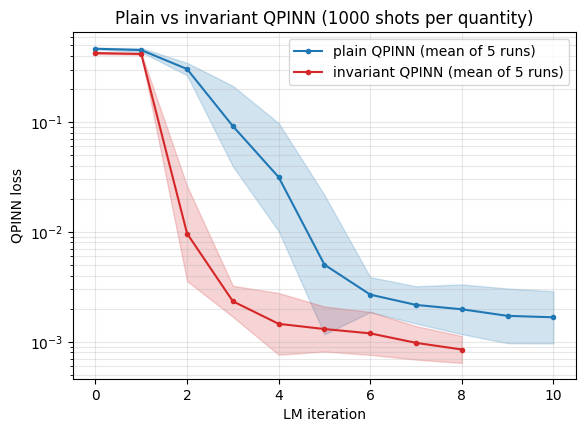
\includegraphics[width=0.82\linewidth]{loss.png}\par
{\tiny Loss per LM step, mean $\pm$ std over 5 runs.\par}

\vspace{0.2ex}
\scriptsize
\setlength{\tabcolsep}{2pt}
\begin{tabular}{@{}lcc@{}}
\toprule
 & plain & \textbf{invariant} \\
\midrule
final loss ($\times10^{-3}$)                    & $1.9\pm0.9$ & $\mathbf{0.9\pm0.3}$ \\
max error $|u_\theta-u^\ast|$ ($\times10^{-2}$) & $4.0\pm1.4$ & $\mathbf{3.4\pm0.3}$ \\
total shots                                     & 896k & \textbf{704k} \\
\bottomrule
\end{tabular}

\vspace{0.4ex}
\raggedright
{\scriptsize LM optimizer stops automatically with the criteria set by us, so the two models run different numbers of iterations.\par}
\vspace{0.6ex}
\footnotesize
\head{Why it matters}
The invariant model performs clearly better
(\textcolor{good}{\textbf{$-$53\,\% loss, $-$21\,\% shots}}),
and this advantage can carry over to many other problems with symmetries\textsuperscript{1}.
\end{column}
\end{columns}
\end{frame}

% =====================================================================
\begin{frame}[c]
\frametitle{Experience with QoolQit}
\framesubtitle{2 \;|\; QoolQit v\qversion}
\small
{\large\textbf{QoolQit version used: v\qversion}}\par
\vspace{2ex}
% ---------------- positive ----------------
\head[good]{\large + \;Positive aspects}
We usually work with qubit models and knew little about analog quantum computing. The
Hamiltonian in QoolQit can easily be written in terms of Pauli matrices, and QoolQit gives
clear hardware control parameters, which made it easy for us to understand.

\vspace{3ex}
% ---------------- challenge ----------------
\head[warn]{\large -- \;Challenges}
Some algorithms may need classical sampling before each shot to decide the parameters of the
Hamiltonian, e.g. Canonical quantization of neurons\footnote[frame]{A.~He, N.~Liu and M.~M.~Wilde, \emph{Canonical quantization of neurons}, arXiv:2607.05000 (2026).},
doubly stochastic gradient descent
optimizers\footnote[frame]{R.~Sweke \emph{et al.}, \emph{Stochastic gradient descent for hybrid quantum-classical optimization}, Quantum \textbf{4}, 314 (2020).}
and Fourier symmetrization for geometric quantum machine learning\textsuperscript{1}.
QoolQit only runs one fixed Hamiltonian for a number of shots and does not cover this case.
We are also not sure how far the hardware supports such operations, so it is unclear how to
design the quantum algorithm best suited to the hardware. A method in QoolQit to roughly judge its feasibility (e.g., runtime) on current hardware would be great for users.
\end{frame}

\end{document}
